\chapter{水与小生物分子}\label{ch:b1:water-small-molecules}

一立方微米的细菌中约含二百亿个水分子，
其余一切分子合计仅数亿个。水并非
\omterm{def:b1:cell-unit-of-life:cell}{细胞}的背景，而是\omterm{def:b1:cell-unit-of-life:cell}{细胞}的介质：它溶解离子与
糖类，包裹蛋白质与膜中疏油的部分，决定
每种酶所依赖的酸碱度，并在
代谢的半数反应中充当反应物或产物。本章介绍水及其
形成与断裂的弱键，酸、碱与
\omterm{def:b1:water-small-molecules:buffer}{缓冲液}的计算，构成后四章大分子的小分子有机物，
以及\omterm{def:b1:water-small-molecules:atp}{能量通货}——\omterm{def:b1:water-small-molecules:atp}{ATP}，
\omterm{def:b1:cell-unit-of-life:cell}{细胞}借它支付构建这些分子的代价。

\section{水}

\begin{definition}[水分子]\label{def:b1:water-small-molecules:water}
\index{水}
水，$\mathrm{H_2O}$，是一种折线形分子（H--O--H 键角为
$104.5^\circ$），氧原子把共用电子拉向自身，
故它是\emph{极性分子}\index{极性分子}，氧原子带部分负电荷，
两个氢原子带部分正电荷。
每个分子至多可形成四个\emph{氢键}\index{氢键}——
一种静电吸引作用，发生在与电负性原子（O、N）结合的氢原子
与另一电负性原子的孤电子对之间，
其中两个经由其氢原子，两个经由其氧原子。
液态水即由这类键构成的网络，每个键仅维持
约数皮秒。
\end{definition}

\begin{omfigure}
\begin{tikzpicture}[font=\small, line cap=round,
  O/.style={circle, draw, thick, fill=omThm!30, minimum size=8mm, inner sep=0pt},
  H/.style={circle, draw, thick, fill=gray!15, minimum size=5.5mm, inner sep=0pt}]
  % central water molecule
  \node[O] (O) at (0,0) {O};
  \node[H] (H1) at (-0.8,-0.7) {H};
  \node[H] (H2) at (0.8,-0.7) {H};
  \draw[thick] (O) -- (H1); \draw[thick] (O) -- (H2);
  \node[font=\scriptsize, omThm] at (0,0.62) {$\delta^-$};
  \node[font=\scriptsize] at (-1.4,-0.55) {$\delta^+$};
  \node[font=\scriptsize] at (1.4,-0.55) {$\delta^+$};
  % lower-left neighbour (accepts an H bond from H1)
  \node[O] (O2) at (-2.1,-2.3) {O};
  \node[H] (H2a) at (-3.05,-2.55) {H};
  \node[H] (H2b) at (-1.75,-3.3) {H};
  \draw[thick] (O2) -- (H2a); \draw[thick] (O2) -- (H2b);
  \draw[dashed, thick, omDef] (H1) -- (O2);
  % lower-right neighbour
  \node[O] (O3) at (2.1,-2.3) {O};
  \node[H] (H3a) at (3.05,-2.55) {H};
  \node[H] (H3b) at (1.75,-3.3) {H};
  \draw[thick] (O3) -- (H3a); \draw[thick] (O3) -- (H3b);
  \draw[dashed, thick, omDef] (H2) -- (O3);
  % upper-left neighbour (donates an H bond to O)
  \node[H] (H4) at (-1.1,1.55) {H};
  \node[O] (O4) at (-2.0,2.25) {O};
  \node[H] (H4b) at (-2.95,2.6) {H};
  \draw[thick] (O4) -- (H4); \draw[thick] (O4) -- (H4b);
  \draw[dashed, thick, omDef] (H4) -- (O);
  % upper-right neighbour
  \node[H] (H5) at (1.1,1.55) {H};
  \node[O] (O5) at (2.0,2.25) {O};
  \node[H] (H5b) at (2.95,2.6) {H};
  \draw[thick] (O5) -- (H5); \draw[thick] (O5) -- (H5b);
  \draw[dashed, thick, omDef] (H5) -- (O);
  \node[anchor=west, align=left, font=\footnotesize] at (4.0,1.0) {虚线：氢键 \\（\qty{0.18}{nm}，每个约\qty{20}{kJ/mol}）\\ 实线：共价 O--H 键 \\（\qty{0.096}{nm}，\qty{460}{kJ/mol}）};
  \node[anchor=west, align=left, font=\footnotesize] at (4.0,-1.3) {每个分子给出两个氢键、接受两个：\\ 四面体网络};
\end{tikzpicture}

{\small 一个水分子（H--O--H 键角 $104.5^\circ$）及其四个
\omterm{def:b1:water-small-molecules:water}{氢键}相连的邻居。这个极性折线形分子通过其氢原子给出两个\omterm{def:b1:water-small-molecules:water}{氢键}，
并通过其氧原子接受两个；由它们形成的网络赋予水
内聚性、热容以及作为溶剂的能力。}
\end{omfigure}

\begin{proposition}[对生命至关重要的水的性质]\label{prop:b1:water-small-molecules:properties}
\omterm{def:b1:water-small-molecules:water}{氢键}网络解释了水的一系列特殊性质：
\begin{itemize}
  \item 较高的\emph{内聚性}与表面张力（\qty{72}{mN/m}）：
        水柱能被拉上树干而不断裂，
        （见\cref{ch:b1:plant-transport}）；昆虫可在池塘水面上行走；
  \item 较高的\emph{热容}（\qty{4.18}{kJ.kg^{-1}.K^{-1}}）
        和较高的汽化热（\qty{2.4}{kJ/g}）：\omterm{def:b1:organism-environment:organism}{生物体}与水体的温度
        变化缓慢，蒸发
        一克汗液即可带走\qty{2.4}{kJ}；
  \item 一种\emph{密度小于液体的固体}：冰会漂浮，而且
        湖泊自上而下凝固，下方留有液态水；
  \item 对离子和\omterm{def:b1:water-small-molecules:water}{极性分子}而言是出色的\emph{溶剂}，
        它以定向排列的壳层将其包围（\emph{水合}）；对非\omterm{def:b1:water-small-molecules:water}{极性分子}则是较差的溶剂，
        它会迫使这类分子聚集在一起（
        \emph{疏水效应}\index{疏水效应}）。
\end{itemize}
\end{proposition}
\begin{proof}[部分证明]
内聚性与表面张力度量的是分离分子所做的功，这些分子各由四个
约\qty{20}{kJ/mol}的键维系。加热
水时必须在打断键的同时使分子剧烈运动，由此产生热容；汽化时则须
将所有键全部打断。冰中每个分子都处于
由四个键构成的开放四面体晶格，其占据的体积大于
无序液体，其中分子排列得更紧密。离子
和极性基团借与水形成的\omterm{def:b1:water-small-molecules:water}{氢键}而得以稳定；非\omterm{def:b1:water-small-molecules:water}{极性
分子}无法形成这类\omterm{def:b1:water-small-molecules:water}{氢键}，其周围的水只得自行排列成笼状结构，
这需付出熵的代价；非\omterm{def:b1:water-small-molecules:water}{极性分子}聚集、共享同一笼状结构时，
此代价便会降低。
\end{proof}

\begin{omfigure}
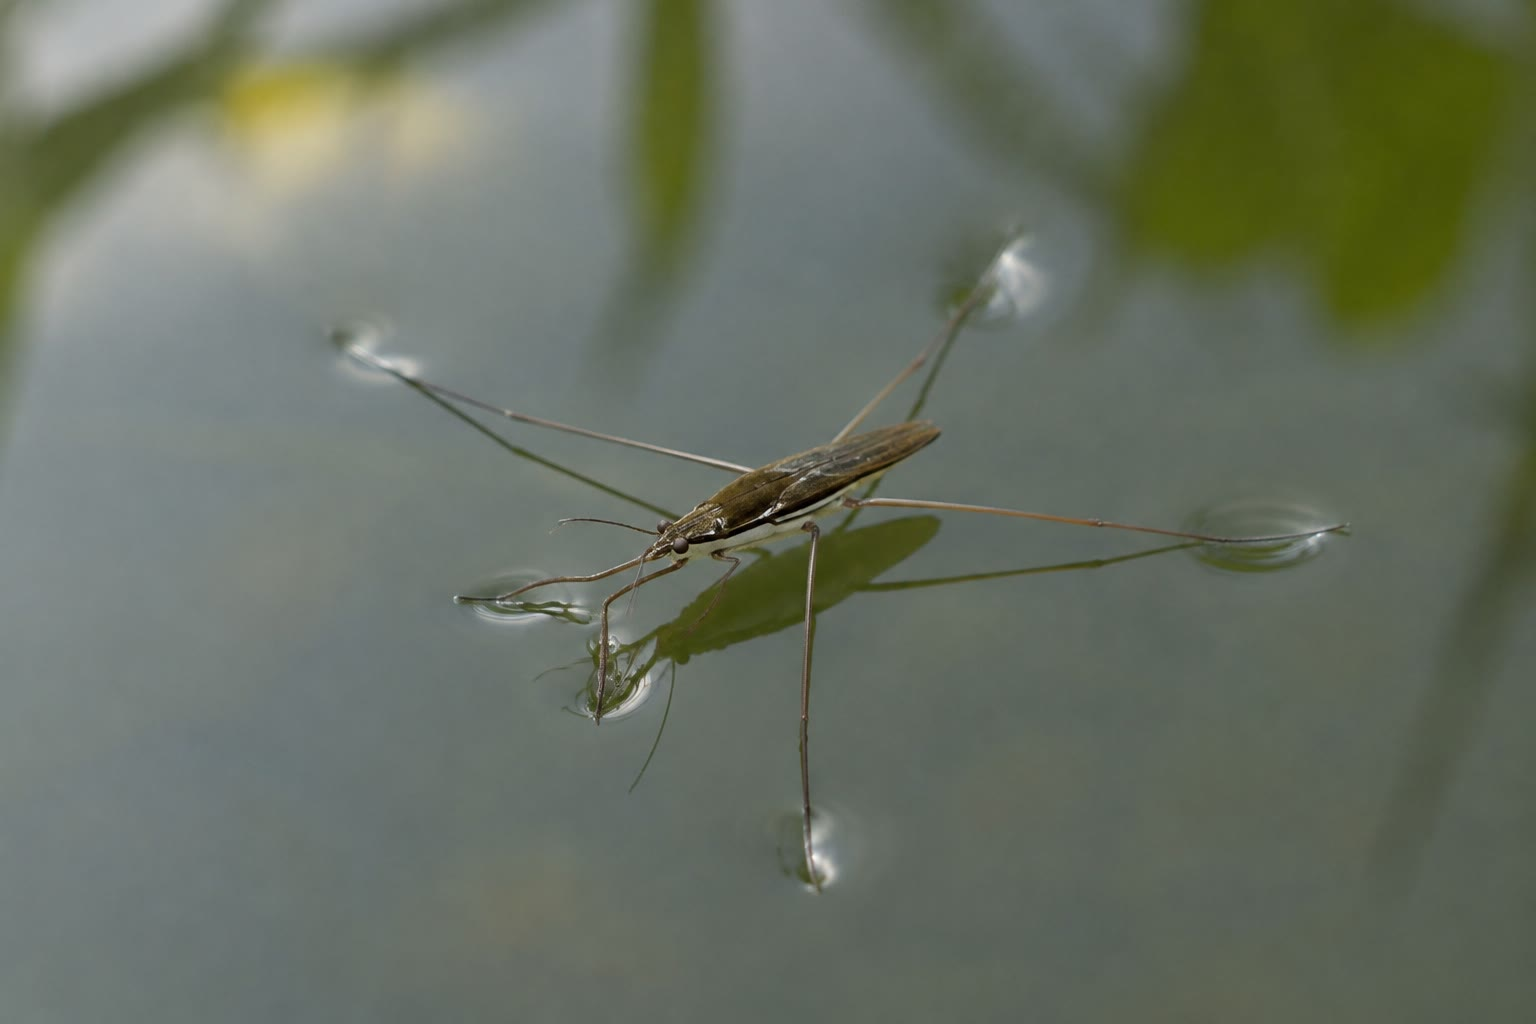
\includegraphics[width=0.6\linewidth]{images/book3/ai/b3-08-water-strider.jpg}

{\small 池塘上的水黾，其足下的凹陷即是
由\omterm{def:b1:water-small-molecules:water}{氢键}结合的水的内聚性所绷紧的水面。}
\end{omfigure}

\begin{example}[疏水效应的作用]\label{ex:b1:water-small-molecules:hydrophobic}
把油倒入水中，几分钟内油滴便已合并：水
会把无法与之成键的物质挤出去。同一效应使蛋白质折叠
（其油性残基藏于内部，见\cref{ch:b1:proteins}），并使
膜组装（脂质的尾部聚集、远离水，
见\cref{ch:b1:lipids}），还促使两个相配的分子表面
相互靠拢。并非油吸引油，而是水在推。
\end{example}

\section{弱键}

\begin{definition}[共价键与非共价键]\label{def:b1:water-small-molecules:bonds}
\emph{共价键}\index{共价键}在两个原子之间共享一对电子，
断开它需 \qtyrange{300}{500}{kJ/mol}：分子的
骨架是共价的，\omterm{def:b1:cell-unit-of-life:cell}{细胞}中只有酶能形成或断开它们。
\emph{非共价键}\index{非共价键}是较弱、可逆的吸引作用，
使分子\emph{彼此}结合并使其成形：
\emph{\omterm{def:b1:water-small-molecules:water}{氢键}}（\qtyrange{4}{20}{kJ/mol}
，水中）；\emph{离子键}\index{离子键}是相反电荷之间的
作用（水中约 \qty{12}{kJ/mol}，水的介电常数
使电荷间作用减弱为八十分之一）；\emph{范德华}\index{范德华}是任意两个紧密接触的原子之间的吸引
（每对 \qtyrange{1}{4}{kJ/mol}，但对整个表面求和）；以及
\emph{\omterm{prop:b1:water-small-molecules:properties}{疏水效应}}，它并非一种键，而是水对
非极性表面的排斥。
\end{definition}

\begin{proposition}[为何弱键是生命的键]\label{prop:b1:water-small-molecules:weak}
在 \qty{37}{\celsius} 时，热能为 $RT = \qty{2.6}{kJ/mol}$。一个
弱键的能量仅为此值的数倍，并在
数微秒内断开；十个弱键同时作用于两个相配的表面，则可维持数小时。
分子\emph{识别}\index{分子识别}——酶与其底物、抗体与其抗原、
以及一条 DNA 链与其互补链——依赖于
互补表面之间同时形成的许多弱键，
这使其既具专一性（只有相配的表面能形成全部弱键），
又具可逆性（加热或竞争者都能使其解除）。
\omterm{def:b1:water-small-molecules:bonds}{共价键}强一百倍，则将是永久的。
\end{proposition}

\begin{example}[双螺旋的熔化]\label{ex:b1:water-small-molecules:melting}
DNA 的两条链由每个碱基对的两个或三个\omterm{def:b1:water-small-molecules:water}{氢键}，
加上相邻碱基对之间的堆积（\omterm{def:b1:water-small-molecules:bonds}{范德华}）作用维系在一起；单个
碱基对会立即分开，而连续排列的一千个碱基对会一直保持
相连，直到温度升至约 \qty{90}{\celsius}，降温时便又以
完全相同的对位重新结合，
（见\cref{ch:b1:nucleic-acids}）。专一、数量多则总体强、可逆。
\end{example}

\section{酸、碱与缓冲液}

\begin{definition}[pH、酸、碱、p$K_a$]\label{def:b1:water-small-molecules:ph}
水会微弱地解离，$\mathrm{H_2O} \rightleftharpoons
\mathrm{H^+} + \mathrm{OH^-}$，且 $[\mathrm{H^+}][\mathrm{OH^-}] =
K_w = \qty{e-14}{mol^2/L^2}$（\qty{25}{\celsius} 时）。
\emph{pH}\index{pH} 为 $-\log_{10}[\mathrm{H^+}]$：纯水为 7，
酸性时更低，碱性时更高。一种\emph{酸}\index{酸} $\mathrm{HA}$
释放一个质子，$\mathrm{HA} \rightleftharpoons \mathrm{H^+} +
\mathrm{A^-}$，其解离常数为 $K_a =
[\mathrm{H^+}][\mathrm{A^-}]/[\mathrm{HA}]$，且
\emph{p$K_a$}\index{pKa@p$K_a$} $= -\log_{10}K_a$；其共轭
\emph{碱}\index{碱} $\mathrm{A^-}$ 可接受一个质子。强酸
（HCl）完全解离；\omterm{def:b1:cell-unit-of-life:cell}{细胞}中的酸（羧酸、
磷酸基团、铵离子）均为弱酸，p$K_a$ 介于 2 与 10 之间。
\end{definition}

\begin{theorem}[亨德森–哈塞尔巴尔赫]\label{thm:b1:water-small-molecules:hh}
\index{亨德森–哈塞尔巴尔赫方程}
对于溶液中的弱酸，
\[
\mathrm{pH} = \mathrm{p}K_a + \log_{10}\frac{[\mathrm{A^-}]}{[\mathrm{HA}]} .
\]
当 $\mathrm{pH} = \mathrm{p}K_a$ 时，酸有一半解离；\omterm{def:b1:water-small-molecules:ph}{pH} 高出
一个单位时，解离度为 \qty{91}{\%}；低一个单位时为 \qty{9}{\%}。
\end{theorem}
\begin{proof}
对 $K_a = [\mathrm{H^+}][\mathrm{A^-}]/[\mathrm{HA}]$ 取对数：
$\log K_a = \log[\mathrm{H^+}] + \log([\mathrm{A^-}]/[\mathrm{HA}])$,
即 $-\mathrm{p}K_a = -\mathrm{pH} + \log([\mathrm{A^-}]/[\mathrm{HA}])$。
比值为 $1$、$10$ 和 $0.1$，分别对应 \omterm{def:b1:water-small-molecules:ph}{pH} $= \mathrm{p}K_a$、$\mathrm{p}K_a + 1$
和 $\mathrm{p}K_a - 1$ 处。
\end{proof}

\begin{definition}[缓冲液]\label{def:b1:water-small-molecules:buffer}
\emph{缓冲液}\index{缓冲液}是一种溶液，其中含有一种弱酸及
其共轭碱，二者量相当；它能抵抗 \omterm{def:b1:water-small-molecules:ph}{pH} 的变化，
因为所加入的 $\mathrm{H^+}$ 会被 $\mathrm{A^-}$ 结合，所加入的
$\mathrm{OH^-}$ 则被 $\mathrm{HA}$ 结合。其效果在
p$K_a$ 上下一个单位内最好，且其\emph{容量}随该
对的总浓度增大而增大。\omterm{def:b1:cell-unit-of-life:cell}{细胞}中的缓冲液有：磷酸基团
（$\mathrm{H_2PO_4^-}/\mathrm{HPO_4^{2-}}$，p$K_a$ 为 6.8）以及
\omterm{def:b1:cell-unit-of-life:cell}{细胞}内蛋白质的侧链；碳酸氢盐（$\mathrm{CO_2}/\mathrm{HCO_3^-}$，
有效 p$K_a$ 为 6.1），存在于血液中，其酸组分是
肺能够排出的一种气体。
\end{definition}

\begin{omfigure}
\begin{tikzpicture}
\begin{axis}[
  width=0.86\linewidth, height=6.2cm,
  axis x line=bottom, axis y line=left,
  xmin=0, xmax=1, ymin=3, ymax=11,
  xlabel={酸的中和分数（所加 $\mathrm{OH^-}$ 的当量）}, ylabel={pH},
  xlabel style={font=\small, at={(axis description cs:0.5,-0.12)}, anchor=north},
  ylabel style={font=\small},
  tick label style={font=\small}, xtick={0,0.25,0.5,0.75,1}, ytick={3,4,5,6,7,8,9,10,11},
  clip=false,
]
\addplot[very thick, omDef, domain=0.02:0.98, samples=120] {6.8 + log10(x/(1-x))};
\draw[dashed, gray] (axis cs:0,6.8) -- (axis cs:0.5,6.8);
\draw[dashed, gray] (axis cs:0.5,3) -- (axis cs:0.5,6.8);
\node[font=\scriptsize, anchor=south west] at (axis cs:0.02,6.85) {pH $=$ p$K_a$ $= 6.8$ 时中和一半};
\draw[<->, thick, omThm] (axis cs:0.09,5.8) -- (axis cs:0.91,7.8);
\node[font=\scriptsize, omThm, anchor=north west, align=left] at (axis cs:0.55,5.7) {缓冲范围：\\ p$K_a \pm 1$，曲线平缓};
\end{axis}
\end{tikzpicture}

{\small 用碱滴定弱酸（磷酸盐，p$K_a$ 6.8）。曲线在
p$K_a$ 附近平缓：此时加入碱只改变碱与酸的比值，\omterm{def:b1:water-small-molecules:ph}{pH} 几乎不变，
超出该范围后，\omterm{def:b1:water-small-molecules:ph}{pH} 变化剧烈。}
\end{omfigure}

\begin{omfigure}
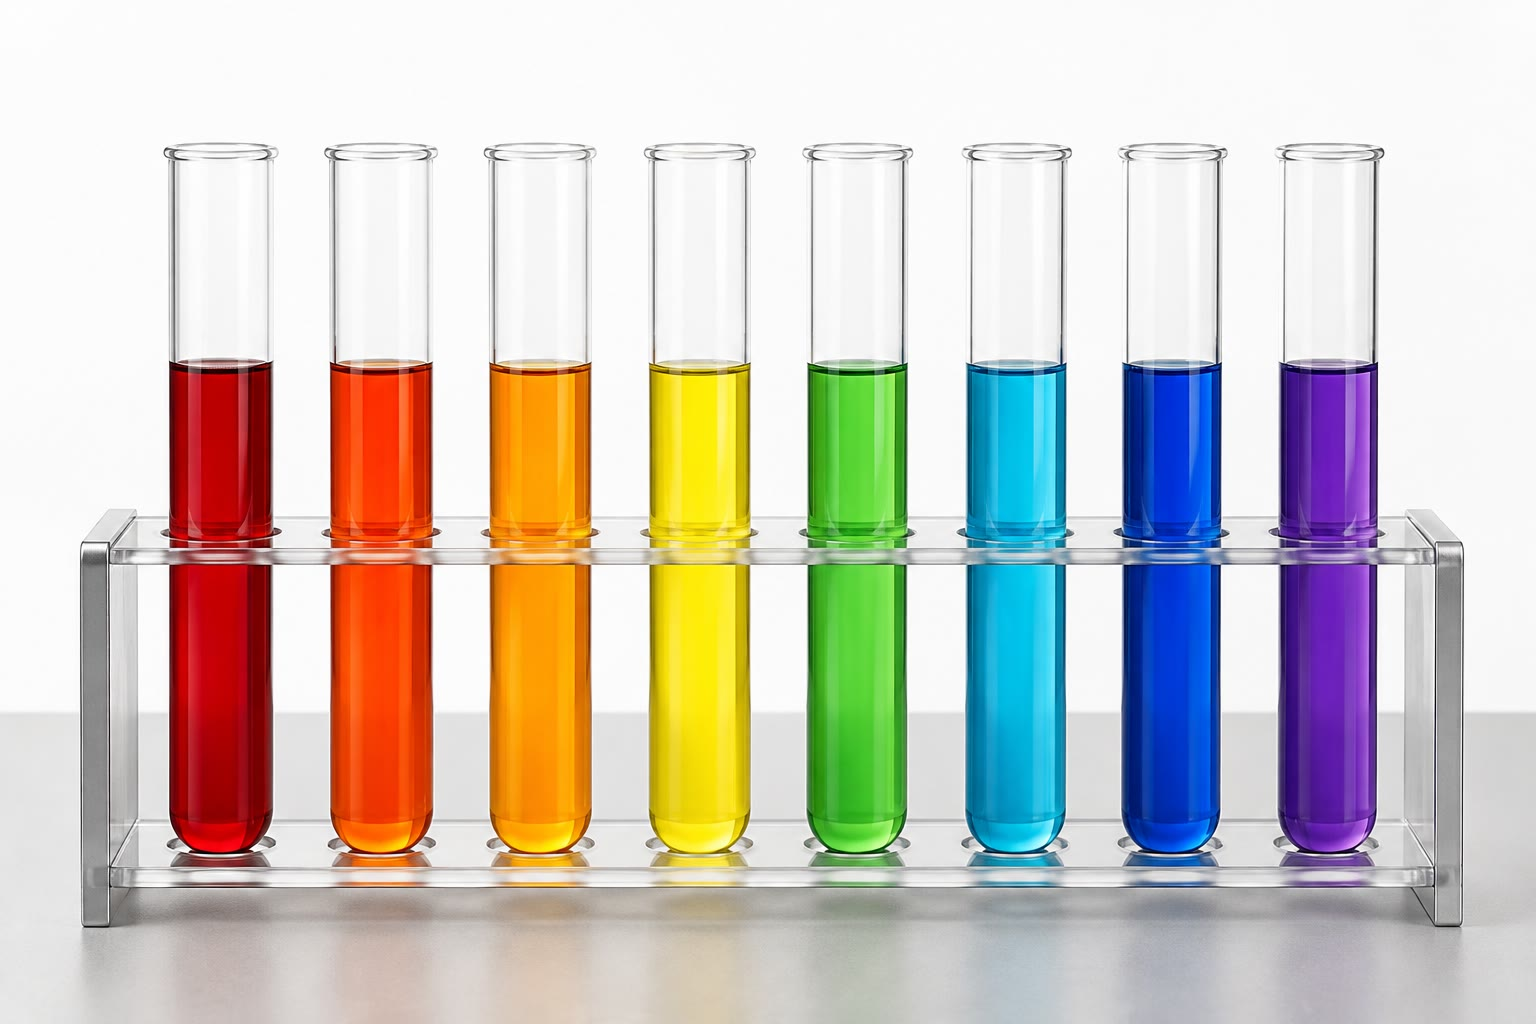
\includegraphics[width=0.6\linewidth]{images/book3/ai/b3-08-indicator-tubes.jpg}

{\small 以通用指示剂呈现的 \omterm{def:b1:water-small-molecules:ph}{pH} 标度：\omterm{def:b1:water-small-molecules:ph}{pH} 2 时为红色，\omterm{def:b1:water-small-molecules:ph}{pH} 12 时为紫色。胃液的 \omterm{def:b1:water-small-molecules:ph}{pH} 为 1--2，
尿液为 5--8，血液为 7.4，小肠为 8，\omterm{def:b1:eukaryotic-cell:organelle}{细胞溶胶}为 7.2，
\omterm{def:b1:eukaryotic-cell:endomembrane}{溶酶体}为 5，光照下\omterm{def:b1:eukaryotic-cell:plastid}{类囊体}腔为 5，
基质为 8。}
\end{omfigure}

\begin{method}[缓冲液计算]\label{met:b1:water-small-molecules:bufferarith}
\begin{enumerate}
  \item 确定酸碱对，并查出其在工作温度下的
        p$K_a$。
  \item 应用 Henderson--Hasselbalch 方程，由 \omterm{def:b1:water-small-molecules:ph}{pH} 求碱与酸的比值，
        或由浓度求 \omterm{def:b1:water-small-molecules:ph}{pH}。
  \item 加入强酸时：从碱中减去其物质的量，
        并将其加到酸中，然后重新计算 \omterm{def:b1:water-small-molecules:ph}{pH}。
        加入强碱时则相反。
  \item 若其中一种组分可离开体系（如呼出二氧化碳、排出氨），
        则该体系为\emph{\omterm{def:b1:organism-environment:organism}{开口系统}}：应将该组分保持在设定值，
        而不让其积累。
        开口\omterm{def:b1:water-small-molecules:buffer}{缓冲液}维持 \omterm{def:b1:water-small-molecules:ph}{pH} 的能力远强于封闭\omterm{def:b1:water-small-molecules:buffer}{缓冲液}。
\end{enumerate}
\end{method}

\begin{example}[血液]\label{ex:b1:water-small-molecules:blood}
动脉血含有 \qty{24}{mmol/L} 的碳酸氢盐和溶解的
$\mathrm{CO_2}$，浓度为 \qty{1.2}{mmol/L}（由肺调节）：$\mathrm{pH} =
6.1 + \log(24/1.2) = 6.1 + 1.30 = 7.4$。加入 \qty{5}{mmol/L} 的酸后，
有 \qty{5}{mmol/L} 的碳酸氢盐转化为 $\mathrm{CO_2}$；若肺将该 $\mathrm{CO_2}$
呼出并保持溶解量不变，则 \omterm{def:b1:water-small-molecules:ph}{pH}
变为 $6.1 + \log(19/1.2) = 7.30$；在封闭烧瓶中，$\mathrm{CO_2}$
将升至 \qty{6.2}{mmol/L}，\omterm{def:b1:water-small-molecules:ph}{pH} 降至 $6.1 + \log(19/6.2) =
6.59$。由此可见，肺起着关键作用。
\end{example}

\section{小分子生物分子}

\begin{definition}[官能团]\label{def:b1:water-small-molecules:groups}
\omterm{def:b1:cell-unit-of-life:cell}{细胞}中的有机分子是碳骨架，其上连接着
一小类\emph{官能团}\index{官能团}，
它们决定了分子的化学性质：
\begin{center}
\small
\begin{tabular}{llll}
\hline
基团 & 化学式 & 性质 & 存在于 \\
\hline
羟基 & $-\mathrm{OH}$ & 极性，可形成\omterm{def:b1:water-small-molecules:water}{氢键} & 糖类，醇 \\
羰基 & $>\!\mathrm{C{=}O}$ & 极性，有反应活性 & 醛糖，酮糖 \\
羧基 & $-\mathrm{COOH}$ & 酸性（p$K_a \approx 4$） & 脂肪酸，氨基酸 \\
氨基 & $-\mathrm{NH_2}$ & 碱性（p$K_a \approx 9$） & 氨基酸 \\
磷酸基 & $-\mathrm{OPO_3^{2-}}$ & 带电，含高能连接 & 核苷酸，\omterm{def:b1:water-small-molecules:atp}{ATP} \\
巯基 & $-\mathrm{SH}$ & 可形成 S--S 键 & 半胱氨酸 \\
甲基 & $-\mathrm{CH_3}$ & 非极性 & 脂质，DNA 标记 \\
\hline
\end{tabular}
\end{center}
在\omterm{def:b1:cell-unit-of-life:cell}{细胞}的 \omterm{def:b1:water-small-molecules:ph}{pH} 条件下，羧基发生电离（$-\mathrm{COO^-}$），
氨基则被质子化（$-\mathrm{NH_3^+}$）。
\end{definition}

\begin{proposition}[四类构件分子]\label{prop:b1:water-small-molecules:families}
\omterm{def:b1:cell-unit-of-life:cell}{细胞}中几乎全部有机物都由四类小分子构成，
每个分子的质量仅为几百道尔顿：\emph{糖类}
(\cref{ch:b1:carbohydrates})、\emph{脂肪酸} (\cref{ch:b1:lipids})、
\emph{氨基酸} (\cref{ch:b1:proteins}) 和\emph{核苷酸}
(\cref{ch:b1:nucleic-acids})。其中三类可连接成
\emph{聚合物}——多糖、蛋白质、核酸——，连接方式为
\emph{缩合}\index{缩合}（形成键时失去一分子水），
并可经\emph{水解}\index{水解}（加入水使键断裂）拆开。
\omterm{prop:b1:water-small-molecules:families}{缩合}为吸能反应，需由 \omterm{def:b1:water-small-molecules:atp}{ATP} 提供能量；
水解为放能反应，只需酶即可进行。
\end{proposition}

\begin{omfigure}
\begin{tikzpicture}[font=\small, >=Stealth, line cap=round,
  mono/.style={draw, thick, rounded corners=3pt, minimum width=16mm, minimum height=8mm, fill=omDef!12}]
  \node[mono] (a) at (0,0) {单体};
  \node[mono] (b) at (2.4,0) {单体};
  \node[font=\footnotesize] at (1.2,0.55) {$-\mathrm{OH}$ \quad $\mathrm{H}-$};
  \draw[->, very thick, omExo] (3.6,0.15) -- (5.6,0.15) node[midway, above, font=\footnotesize, align=center] {缩合 \\ （消耗 ATP）};
  \draw[->, very thick, omThm] (5.6,-0.15) -- (3.6,-0.15) node[midway, below, font=\footnotesize, align=center] {水解 \\ （仅需酶）};
  \node[mono, minimum width=34mm] (ab) at (7.6,0) {单体——单体};
  \node[font=\footnotesize] at (7.6,0.55) {共价连接};
  \node[font=\footnotesize, omDef] at (9.9,-0.6) {$+\ \mathrm{H_2O}$};
\end{tikzpicture}

{\small \omterm{prop:b1:water-small-molecules:families}{缩合}使两个构件连接起来并失去一分子水；水解则通过加入一分子水将其拆开。
糖类、氨基酸和核苷酸
均以此方式聚合。}
\end{omfigure}

\begin{example}[细胞的组成]\label{ex:b1:water-small-molecules:inventory}
在细菌的干质量中，蛋白质占 \qty{55}{\%}，RNA 占 \qty{20}{\%}，
DNA 占 \qty{3}{\%}，脂质占 \qty{9}{\%}，多糖占 \qty{5}{\%}，
其余为小分子和离子。若按分子数计，情况则截然相反：
约一千种小分子代谢物和离子，
浓度从纳摩尔到每升十分之一摩尔不等，
构成了非水分子中的绝大多数。
钾离子浓度为 \qty{150}{mmol/L}，谷氨酸为 \qty{100}{mmol/L}，
\omterm{def:b1:water-small-molecules:atp}{ATP} 为 \qty{5}{mmol/L}，转录因子则仅有每个\omterm{def:b1:cell-unit-of-life:cell}{细胞}几个分子。
\end{example}

\section{能量：自由能与 ATP}

\begin{proposition}[恒温恒压下反应的自由能]\label{prop:b1:water-small-molecules:gibbs}
\index{自由能}
在恒温恒压下，反应会自发地
朝着使吉布斯\omterm{prop:b1:water-small-molecules:gibbs}{自由能} $G$ 降低的方向进行。对于
$\mathrm{A} + \mathrm{B} \rightleftharpoons \mathrm{C} + \mathrm{D}$，
\[
\Delta G = \Delta G^{\circ\prime} + RT\ln\frac{[\mathrm{C}][\mathrm{D}]}{[\mathrm{A}][\mathrm{B}]},
\]，
其中 $\Delta G^{\circ\prime}$ 为标准\omterm{prop:b1:water-small-molecules:gibbs}{自由能}变化
（所有浓度均为 \qty{1}{mol/L}，\omterm{def:b1:water-small-molecules:ph}{pH} 为 7），而对数项
则对实际浓度加以修正。平衡时 $\Delta G = 0$，
因此 $\Delta G^{\circ\prime} = -RT\ln K'_{\text{eq}}$：每
$\Delta G^{\circ\prime}$ 改变 \qty{5.7}{kJ/mol}，平衡常数便变为原来的十倍。
$\Delta G$ 说明反应能够朝哪个方向进行，
而反应快慢则取决于酶（见\cref{ch:b1:enzymes}）。
\end{proposition}
\begin{proof}
每种物质的化学势为 $\mu = \mu^\circ + RT\ln c$
（即物理课程中理想溶液的结果）；$\Delta G$ 等于产物化学势之和
减去反应物化学势之和，由此得到上式；令其在平衡时
为零，即可得到与
$K'_{\text{eq}}$ 的关系。
\end{proof}

\begin{definition}[ATP、偶联]\label{def:b1:water-small-molecules:atp}
\emph{ATP}\index{ATP}（三磷酸腺苷）是一种核苷酸
（见\cref{ch:b1:nucleic-acids}），其上依次连有三个磷酸基团；外侧两个键为
\emph{磷酸酐键}\index{磷酸酐键}，
其水解反应 $\mathrm{ATP} + \mathrm{H_2O} \to \mathrm{ADP} +
\mathrm{P_i}$ 的 $\Delta G^{\circ\prime} = \qty{-30.5}{kJ/mol}$，
在\omterm{def:b1:cell-unit-of-life:cell}{细胞}内浓度条件下 $\Delta G \approx \qty{-50}{kJ/mol}$。
ATP 是\omterm{def:b1:cell-unit-of-life:cell}{细胞}的\emph{能量通货}\index{能量通货}：
分解代谢产生 ATP（见\cref{ch:b1:respiration-fermentation}），
生物合成、运输和运动则消耗 ATP。吸能反应
需通过\emph{偶联}\index{偶联}借 ATP 水解才能进行，
即经由一个共同的中间产物与之连接，
使两个反应的 $\Delta G$ 之和为负。
\end{definition}

\begin{example}[为什么 ATP 水解释放这么多能量]\label{ex:b1:water-small-molecules:whyatp}
原因有三：\omterm{def:b1:water-small-molecules:atp}{ATP} 磷酸基团上的四个负电荷彼此排斥，断键后
这种排斥得以缓解；产物 $\mathrm{ADP}$ 和 $\mathrm{P_i}$ 比酸酐
更能通过共振和水合作用稳定；此外，\omterm{def:b1:cell-unit-of-life:cell}{细胞}使 \omterm{def:b1:water-small-molecules:atp}{ATP} 的浓度保持
在高于其与 ADP 及磷酸平衡浓度约一千倍的水平。
其中最后一点影响最大：
若 \omterm{def:b1:water-small-molecules:atp}{ATP} 为 \qty{5}{mmol/L}，ADP 为 \qty{1}{mmol/L}，$\mathrm{P_i}$
为 \qty{10}{mmol/L}，
$\Delta G = -30.5 + 2.58\ln\frac{10^{-3}\times 10^{-2}}{5\times 10^{-3}}
= -30.5 - 16 = \qty{-46.5}{kJ/mol}$。
\end{example}

\begin{example}[偶联]\label{ex:b1:water-small-molecules:coupling}
葡萄糖 $+\ \mathrm{P_i} \to$ 6-磷酸葡萄糖 $+\ \mathrm{H_2O}$
的 $\Delta G^{\circ\prime} = \qty{+13.8}{kJ/mol}$：平衡时
几乎没有葡萄糖会被磷酸化。己糖激酶则
直接从 \omterm{def:b1:water-small-molecules:atp}{ATP} 转移磷酸基团：葡萄糖 $+$ \omterm{def:b1:water-small-molecules:atp}{ATP} $\to$
6-磷酸葡萄糖 $+$ ADP，$\Delta G^{\circ\prime} = 13.8 - 30.5 =
\qty{-16.7}{kJ/mol}$，平衡常数为 $800$，反应基本进行到底。
磷酸基团从不以游离形式出现：两步反应实为一步。
\end{example}

\section{练习}

\begin{exercise}[$\star$]\label{exo:b1:water-small-molecules:1}
从水分子的结构出发，解释为什么水是盐的良好溶剂，
而是油的不良溶剂。
\end{exercise}

\begin{exercise}[$\star$]\label{exo:b1:water-small-molecules:2}
按强度对四类非共价相互作用排序，
并分别给出其一种生物学作用。
\end{exercise}

\begin{exercise}[$\star$]\label{exo:b1:water-small-molecules:3}
计算 $[\mathrm{H^+}] = \qty{4e-8}{mol/L}$ 的溶液的 \omterm{def:b1:water-small-molecules:ph}{pH}，
并求 \omterm{def:b1:water-small-molecules:ph}{pH} 为 1.5 的胃液中的 $[\mathrm{H^+}]$。
\end{exercise}

\begin{exercise}[$\star$]\label{exo:b1:water-small-molecules:4}
由滴定曲线图，磷酸盐\omterm{def:b1:water-small-molecules:buffer}{缓冲液}在哪一 \omterm{def:b1:water-small-molecules:ph}{pH} 范围内起作用？
\omterm{def:b1:water-small-molecules:ph}{pH} 为 7.4 时，碱与酸的比值是多少？
\end{exercise}

\begin{exercise}[$\star\star$]\label{exo:b1:water-small-molecules:5}
乙酸的 p$K_a$ 为 4.76。求乙酸在 \omterm{def:b1:water-small-molecules:ph}{pH} 4.76、
\omterm{def:b1:water-small-molecules:ph}{pH} 7.2（\omterm{def:b1:eukaryotic-cell:organelle}{细胞溶胶}）和 \omterm{def:b1:water-small-molecules:ph}{pH} 2（胃）时的解离比例。哪种形式
更容易穿过膜？乙酸应在何处被吸收？
\end{exercise}

\begin{exercise}[$\star\star$]\label{exo:b1:water-small-molecules:6}
某\omterm{def:b1:water-small-molecules:buffer}{缓冲液}含有 \qty{50}{mmol/L} 的 $\mathrm{HPO_4^{2-}}$ 和
\qty{50}{mmol/L} 的 $\mathrm{H_2PO_4^-}$（p$K_a$ 为 6.8）。计算其 \omterm{def:b1:water-small-molecules:ph}{pH}。
计算加入 \qty{10}{mmol/L} 的 HCl 后的 \omterm{def:b1:water-small-molecules:ph}{pH}，
并计算在纯水中加入相同 HCl 后的 \omterm{def:b1:water-small-molecules:ph}{pH}。
\end{exercise}

\begin{exercise}[$\star\star$]\label{exo:b1:water-small-molecules:7}
汗液蒸发可使跑步者降温。需蒸发多少汗液
才能带走 \qty{500}{kJ} 的热量？请用\omterm{def:b1:water-small-molecules:water}{氢键}解释
水的汽化热为何如此之大。
\end{exercise}

\begin{exercise}[$\star\star$]\label{exo:b1:water-small-molecules:8}
反应葡萄糖-1-磷酸 $\to$ 葡萄糖-6-磷酸在 \qty{25}{\celsius} 下的
$K'_{\text{eq}} = 19$。计算 $\Delta G^{\circ\prime}$。
在某\omterm{def:b1:cell-unit-of-life:cell}{细胞}中，葡萄糖-6-磷酸为 \qty{2}{mmol/L}，
葡萄糖-1-磷酸为 \qty{0.02}{mmol/L}，计算
$\Delta G$，并说明反应朝哪个方向进行。
\end{exercise}

\begin{exercise}[$\star\star$]\label{exo:b1:water-small-molecules:9}
湖泊为何从上往下结冰，这对其中的鱼类
有何意义？若冰会下沉，世界将会怎样？
\end{exercise}

\begin{exercise}[$\star\star\star$]\label{exo:b1:water-small-molecules:10}
计算肌肉\omterm{def:b1:cell-unit-of-life:cell}{细胞}中 \omterm{def:b1:water-small-molecules:atp}{ATP} 水解的 $\Delta G$，其中 \omterm{def:b1:water-small-molecules:atp}{ATP} 为
\qty{8}{mmol/L}，ADP 为 \qty{0.9}{mmol/L}，$\mathrm{P_i}$ 为
\qty{8}{mmol/L}，温度为 \qty{37}{\celsius}；再计算疲劳肌肉中的情况，其中 \omterm{def:b1:water-small-molecules:atp}{ATP} 为
\qty{5}{mmol/L}，ADP 为 \qty{3}{mmol/L}，$\mathrm{P_i}$ 为
\qty{30}{mmol/L}。疲劳对每个 \omterm{def:b1:water-small-molecules:atp}{ATP} 可用的能量产生了
什么影响？
\end{exercise}

\begin{exercise}[$\star\star\star$]\label{exo:b1:water-small-molecules:11}
\omterm{def:b1:cell-unit-of-life:cell}{细胞}在 \omterm{def:b1:water-small-molecules:ph}{pH} 7.2、\qty{37}{\celsius} 下，内部体积为
\qty{1000}{\micro m^3}。该\omterm{def:b1:cell-unit-of-life:cell}{细胞}中含有多少个游离的 $\mathrm{H^+}$ 离子，
与其 $\num{3e9}$ 个缓冲基团相比如何？这一比较说明
“\omterm{def:b1:cell-unit-of-life:cell}{细胞}的 \omterm{def:b1:water-small-molecules:ph}{pH}”一词具有怎样的含义？
\end{exercise}

\begin{exercise}[$\star\star\star$]\label{exo:b1:water-small-molecules:12}
“生命是让反应远离平衡的一种方式。”请用一段话讨论，
结合 \omterm{def:b1:water-small-molecules:atp}{ATP} 的浓度比、\omterm{def:b1:water-small-molecules:atp}{偶联}，以及
其 \omterm{def:b1:water-small-molecules:atp}{ATP} 与 ADP 达到平衡的\omterm{def:b1:cell-unit-of-life:cell}{细胞}会发生什么。
\end{exercise}

\section{问题：血液作为缓冲液}

\begin{problem}[{周末问题——pH 为 7.40 的五升血液经过一次短跑：
碳酸氢根、二氧化碳、肺与肾，
最后求给定乳酸负荷下的 pH 变化}]
\label{pb:b1:water-small-molecules:1}
动脉血：\omterm{def:b1:water-small-molecules:ph}{pH} 7.40，碳酸氢根 $[\mathrm{HCO_3^-}] =
\qty{24}{mmol/L}$，溶解的二氧化碳 $[\mathrm{CO_2}] =
\qty{1.2}{mmol/L}$（与其分压成正比，分压为
\qty{40}{mmHg} 时为 \qty{1.2}{mmol/L}）。碳酸氢根体系
的有效 p$K_a$ 为 6.1：$\mathrm{CO_2} + \mathrm{H_2O}
\rightleftharpoons \mathrm{H^+} + \mathrm{HCO_3^-}$。血液体积为
\qty{5}{L}。\omterm{def:b1:mammal-organization:compartments}{血浆}蛋白与血红蛋白又构成第二种\omterm{def:b1:water-small-molecules:buffer}{缓冲液}，
其容量为每升每 \omterm{def:b1:water-small-molecules:ph}{pH} 单位 \qty{25}{mmol} 的 $\mathrm{H^+}$。一次短跑
会释放 \qty{60}{mmol} 乳酸（在血液
\omterm{def:b1:water-small-molecules:ph}{pH} 下为强酸），并在一分钟内进入血液。

\medskip
\noindent\textbf{第一部分——静息状态。}
\begin{enumerate}
  \item 根据碳酸氢根与二氧化碳的数值，验证
        动脉血的 \omterm{def:b1:water-small-molecules:ph}{pH}。
  \item 计算 \omterm{def:b1:water-small-molecules:ph}{pH} 为 7.40 时的 $[\mathrm{H^+}]$，单位为纳摩尔每升。
  \item 整个血液中共有多少游离质子？
        并与 \qty{120}{mmol} 的碳酸氢根比较。
  \item 计算碳酸氢根与溶解二氧化碳之比，
        以及缓冲对中以碱形式存在的比例。
  \item 静脉血中 $\mathrm{CO_2}$ 的分压为
        \qty{46}{mmHg}，碳酸氢根为 \qty{25}{mmol/L}。计算其
        \omterm{def:b1:water-small-molecules:ph}{pH}。
  \item 为何 p$K_a$ 为 6.1，比血液 \omterm{def:b1:water-small-molecules:ph}{pH} 低一个以上单位，
        在体内对该缓冲体系并非不利，
        而在烧瓶中则是一种不利？
\end{enumerate}

\medskip
\noindent\textbf{第二部分——短跑，封闭系统。}
先假设二氧化碳不能离开血液：碳酸氢根
每结合一个质子，都会转化为溶解的 $\mathrm{CO_2}$。
\begin{enumerate}[resume]
  \item 计算加入血液的乳酸浓度。
  \item 若全部酸均由碳酸氢根缓冲，计算
        新的碳酸氢根与新的溶解 $\mathrm{CO_2}$。
  \item 计算所得的 \omterm{def:b1:water-small-molecules:ph}{pH}。
  \item 计算同样的酸在 \qty{5}{L} 纯
        水中所得的 \omterm{def:b1:water-small-molecules:ph}{pH}。
  \item 封闭的碳酸氢根体系对于此负荷是否为良好的\omterm{def:b1:water-small-molecules:buffer}{缓冲液}？
        用 \omterm{def:b1:water-small-molecules:ph}{pH} 的变化量加以定量。
  \item 计算 $[\mathrm{H^+}]$ 在 \omterm{def:b1:water-small-molecules:ph}{pH} 7.40 与
        第 9 题所得 \omterm{def:b1:water-small-molecules:ph}{pH} 之间的变化，以及加入的质子中
        仍以游离形式留在溶液中的比例。
\end{enumerate}

\medskip
\noindent\textbf{第三部分——短跑，\omterm{def:b1:organism-environment:organism}{开口系统}。}
现在由肺将溶解的 $\mathrm{CO_2}$ 维持在 \qty{1.2}{mmol/L}，
即通过呼出多余部分来实现。
\begin{enumerate}[resume]
  \item 计算碳酸氢根为新值时的 \omterm{def:b1:water-small-molecules:ph}{pH}，
        其中 $\mathrm{CO_2}$ 维持在 \qty{1.2}{mmol/L}。
  \item 为维持该数值，肺须额外排出多少毫摩尔的
        $\mathrm{CO_2}$（超出静息排出量）？
  \item 静息时的排出量为每分钟 \qty{10}{mmol} 的 $\mathrm{CO_2}$。
        通气量须升高到原来的多少倍，
        才能在一分钟内清除多余部分？
  \item 跑者进一步过度通气，使
        $\mathrm{CO_2}$ 的分压降至 \qty{30}{mmHg}，计算新的
        溶解 $\mathrm{CO_2}$ 量及 \omterm{def:b1:water-small-molecules:ph}{pH}。
  \item 现在计入蛋白质\omterm{def:b1:water-small-molecules:buffer}{缓冲液}：在 \qty{60}{mmol} 质子中，
        按两种\omterm{def:b1:water-small-molecules:buffer}{缓冲液}的容量比例，由蛋白质承担一部分，
        估算开口碳酸氢根体系在 \omterm{def:b1:water-small-molecules:ph}{pH} 7.4 附近的容量
        （即每升中使 \omterm{def:b1:water-small-molecules:ph}{pH} 改变一个单位所需的酸的毫摩尔数，
        由 Henderson--Hasselbalch 方程得出，
        在 $\mathrm{CO_2}$ 固定的条件下计算），以及
        各\omterm{def:b1:water-small-molecules:buffer}{缓冲液}所承担的质子份额。
  \item 计算两种\omterm{def:b1:water-small-molecules:buffer}{缓冲液}共同作用下，短跑后的 \omterm{def:b1:water-small-molecules:ph}{pH}。
\end{enumerate}

\medskip
\noindent\textbf{第四部分——恢复与肾脏。}
\begin{enumerate}[resume]
  \item 在接下来的一小时内，肝脏氧化乳酸（清除
        其中的酸），在肺维持 $\mathrm{CO_2}$ 不变的情况下，
        碳酸氢根与 \omterm{def:b1:water-small-molecules:ph}{pH} 会发生什么变化？
  \item 一名肾衰竭患者每天滞留 \qty{60}{mmol} 的酸，
        且无法将其排出。计算碳酸氢根每天的减少量
        （\omterm{def:b1:organism-environment:organism}{开口系统}），以及若碳酸氢根不予补充，
        三天后的 \omterm{def:b1:water-small-molecules:ph}{pH}。
  \item 一名肺病患者滞留的 $\mathrm{CO_2}$ 分压为
        \qty{60}{mmHg}，碳酸氢根为
        \qty{24}{mmol/L}。计算 \omterm{def:b1:water-small-molecules:ph}{pH}。肾脏在数日内
        通过将碳酸氢根提高至 \qty{33}{mmol/L} 作出调节；计算此时的
        \omterm{def:b1:water-small-molecules:ph}{pH}。
  \item 用两句话解释为何肺能在数分钟内校正 \omterm{def:b1:water-small-molecules:ph}{pH}，
        而肾脏需要数日，并说明二者各自控制 Henderson--Hasselbalch
        比值中的哪一部分。
  \item 肾脏通过 \qty{1.5}{L} 尿液排出一天的 \qty{60}{mmol} 酸，
        尿液 \omterm{def:b1:water-small-molecules:ph}{pH} 为 5。计算该尿液中的游离质子数，
        并由此推断酸的运输方式。
  \item 呕吐损失 \qty{100}{mmol} 的 HCl。预测 \omterm{def:b1:water-small-molecules:ph}{pH} 变化的
        方向，并计算\omterm{def:b1:organism-environment:organism}{开口系统}中的 \omterm{def:b1:water-small-molecules:ph}{pH} 变化量。
  \item 给出结论：血液 \omterm{def:b1:water-small-molecules:ph}{pH} 的变化，针对
        \qty{60}{mmol} 乳酸负荷，分别在封闭系统中、
        仅有碳酸氢根的\omterm{def:b1:organism-environment:organism}{开口系统}中，以及加入蛋白质\omterm{def:b1:water-small-molecules:buffer}{缓冲液}后的
        \omterm{def:b1:water-small-molecules:ph}{pH} 变化。
\end{enumerate}
\end{problem}
